\chapter{Auswertungstool zur Gitterstudie}
\label{cha:auswertungstool}
Für die in dieser Ausarbeitung durchgeführten Gitterstudien wurde ein Auswertungstool in Matlab erstellt. Es eignet sich für CFX-Simulationen.\\
Ziel war es eine einfache Bedienung mit wenigen Einstellmöglichkeiten zu ermöglichen. So kann dieses Tool ohne Matlab Kenntnisse genutzt werden.
\image überarbeiten
\begin{figure}[htbp]
	\centering
	\label{fig:auswerungbsp}
	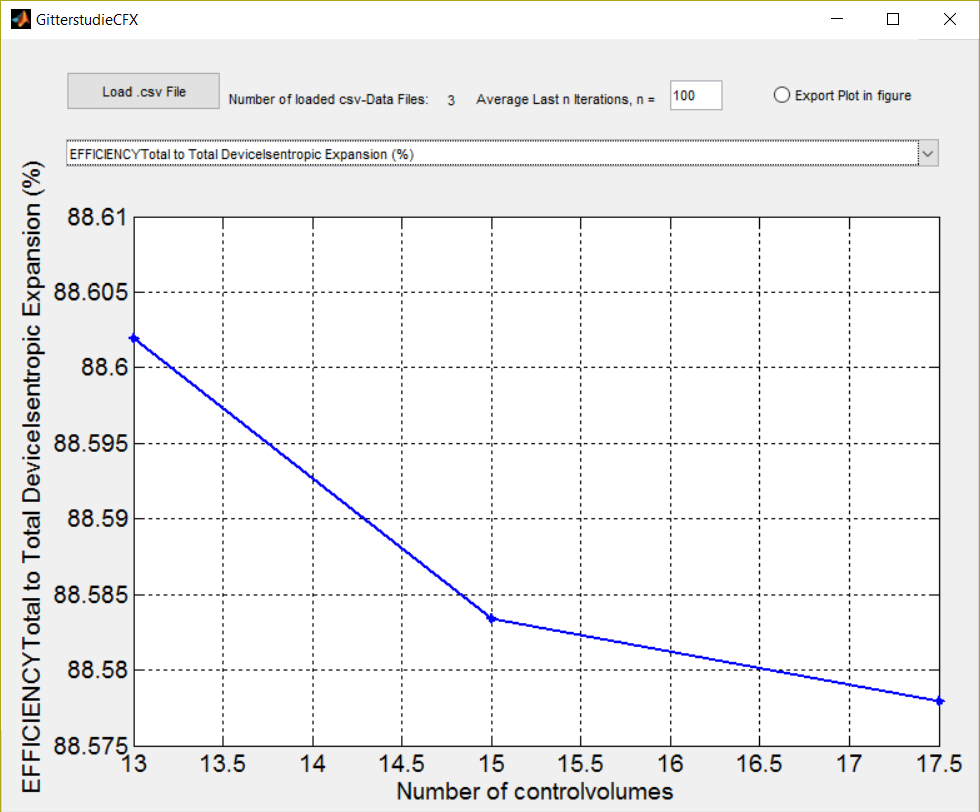
\includegraphics[width=0.8\textwidth]{auswertungstoolbsp.png}
	\caption{Auswertungstool zur Gitterstudie}
\end{figure}

\section{Funktionsumpfang}
\todo

\section{Benutzung}
Um dieses Tool auszuführen muss die Funktion \texttt{GitterstudieCFX} in Matlab ausgeführt werden. Nun können über den Button \textit{Load .csv File} csv-Dateien einzeln eingeladen werden. Diese wurden vorher mit \texttt{cfx5mondata -res filename.res -out filename.csv} erzeugt. In dem sich öffnenden Dialogfenster muss die Kontrollvolumenzahl, beziehungsweise  die Verfeinerungsstufe der eingelesen Datei eingegeben werden. Nach dem Einlesen kann im Drop-Down Menü die darzustellende Größe ausgewählt werden. Über den Export-Button wird das Diagramm in einem Extra-Fenster geöffnet und lässt sich in verschiedenen Formaten abspeichern.
\subsection{Wichtige Hinweise}
\lstset{language=Matlab}
\begin{itemize}
\item Die Dateien müssen von der gröbsten bis zur feinsten Verfeinerung in aufsteigender Reihenfolge eingeladen werden.
\item In den Definitionen der Userpoints in CFX dürfen keine Anführungszeichen verwendet werden. Diese dienen als Trennzeichen in der csv-Datei und führen zu Komplikationen.
\item Die Schriftgröße der Achsenbeschriftung kann unter \texttt{FontSize} in den folgenden Zeilen verändert werden.
\begin{lstlisting}[frame=single]
xlabel('Number of controlvolumes','FontSize',14);
ylabel(...,'FontSize',14);
\end{lstlisting}
\item Die Schriftgröße der Achsen wird ebenfalls mit \texttt{FontSize} eingestellt.
\begin{lstlisting}[frame=single]
set(gca,'FontSize',14);
\end{lstlisting}
\item Die Linienstärke wird  mit \texttt{Linewidth} angepasst.
\begin{lstlisting}[frame=single]
plot(g(:), fPlot(:), '*-b', 'Linewidth',2);
\end{lstlisting}
\item Die Defaultwerte sorgen bereits für eine gute Lesbarkeit in Ausarbeitungen.
\item Dieses Tool mittelt standardmäßig die letzten 100 Iterationen einer Simulation. Dies kann allerdings vor dem Einlesen einer Datei in dem dazugehörigen Textfeld umgestellt werden. 
\end{itemize}

